\ifdefined\ishandout
\documentclass[handout]{beamer}
\else
\documentclass{beamer}
\fi

%\usepackage[frenchb]{babel}
\usepackage[T1]{fontenc}
%\usepackage[utf8]{inputenc}
\usepackage{hyperref}
\usepackage{multirow}
\usepackage{listings}
\usepackage{fancyvrb}
\usepackage{tikz}
\usepackage{framed}
\usepackage{xmpmulti}

\usepackage{algorithm}
\usepackage{algorithmicx}
\usepackage{algpseudocode}
\usepackage{xcolor}
\usepackage{booktabs}
\usepackage{color, colortbl}
\ifdefined\ishandout
\usepackage{handoutWithNotes}
\fi
\usepackage{slashbox}
\usepackage{amsmath}
\usepackage{bm}
\usepackage{hhline}
\usepackage{pgfplots}
\usepackage{caption}

\def\UrlBreaks{\do\/\do-}

\usetikzlibrary{shapes.geometric}
\usetikzlibrary{positioning}
\usetikzlibrary{shapes.arrows, chains}
\usetikzlibrary{arrows,calc}
\usetikzlibrary{shapes.multipart}
\usetikzlibrary{matrix}

\usepackage{array}
%\usetheme{Boadilla}
\usetheme[progressbar=frametitle]{metropolis}

\usefonttheme[onlymath]{serif}

\newcommand{\R}{\mathbb{R}}
%\newcommand{\C}{\mathbb{C}}
\newcommand{\N}{\mathbb{N}}
\newcommand{\Z}{\mathbb{Z}}
\newcommand{\E}{\mathbb{E}}
\newcommand{\Var}{\text{Var}}
\newcommand{\Cov}{\text{Cov}}
\ifdefined\ishandout
\pgfpagesuselayout{3 on 1 with notes}[a4paper,border shrink=5mm]
\usecolortheme{dove}
\else
%\usecolortheme{dolphin}
%\usecolortheme{crane}
\fi

\metroset{block=fill}

\lstnewenvironment{codeC}
{ \lstset{language=C,
    otherkeywords={printf,scanf}}
}
{}

\ifdefined\ishandout
\definecolor{mygreen}{rgb}{0,0,0}
\definecolor{mymauve}{rgb}{0,0,0}
\definecolor{myblue}{rgb}{0,0,0}
\else
\definecolor{mygreen}{rgb}{0,0.6,0}
\definecolor{mymauve}{rgb}{0.58,0,0.82}
\definecolor{myblue}{rgb}{0,0,1}

\fi

%% Notes
%\setbeameroption{show only notes}


\definecolor{mygray}{rgb}{0.5,0.5,0.5}

\lstset{ language=Python,%
  backgroundcolor=\color{white},   % choose the background color; you must add \usepackage{color} or \usepackage{xcolor}
  basicstyle=\footnotesize,        % the size of the fonts that are used for the code
  breakatwhitespace=false,         % sets if automatic breaks should only happen at whitespace
  breaklines=true,                 % sets automatic line breaking
  captionpos=b,                    % sets the caption-position to bottom
  commentstyle=\color{mygreen},    % comment style
  deletekeywords={...},            % if you want to delete keywords from the given language
  escapeinside={\%*}{*)},          % if you want to add LaTeX within your code
  extendedchars=true,              % lets you use non-ASCII characters; for 8-bits encodings only, does not work with UTF-8
  frame=tb,	                   % adds a frame around the code
  keepspaces=true,                 % keeps spaces in text, useful for keeping indentation of code (possibly needs columns=flexible)
  keywordstyle=\color{blue},       % keyword style
  otherkeywords={*,...},           % if you want to add more keywords to the set
  numbers=none,                    % where to put the line-numbers; possible values are (none, left, right)
  numbersep=5pt,                   % how far the line-numbers are from the code
  numberstyle=\tiny\color{mygray}, % the style that is used for the line-numbers
  rulecolor=\color{black},         % if not set, the frame-color may be changed on line-breaks within not-black text (e.g. comments (green here))
  showspaces=false,                % show spaces everywhere adding particular underscores; it overrides 'showstringspaces'
  showstringspaces=false,          % underline spaces within strings only
  showtabs=false,                  % show tabs within strings adding particular underscores
  stepnumber=2,                    % the step between two line-numbers. If it's 1, each line will be numbered
  stringstyle=\color{mymauve},     % string literal style
  tabsize=3,	                   % sets default tabsize to 2 spaces
  title=\lstname                   % show the filename of files included with \lstinputlisting; also try caption instead of title
}
%\lstset{language=Python,
% breakatwhitespace=false,         % sets if automatic breaks should only happen at whitespace
%  breaklines=true,                 % sets automatic line breaking
%  captionpos=b,                
%%commentstyle=\itshape\color{mymauve},
%%keywordstyle=\bfseries\color{myblue},
%numbers=left,                    % where to put the line-numbers; possible values are (none, left, right)
%  numbersep=8pt,                   % how far the line-numbers are from the code
%  numberstyle=\tiny\color{mygray}, % the style that is used for the line-numbers
%%  rulecolor=\color{black},         % if not set, the frame-color may be changed on line-breaks within not-black text (e.g. comments (green here))
%  showspaces=false,                % show spaces everywhere adding particular underscores; it overrides 'showstringspaces'
%%  showstringspaces=false,          % underline spaces within strings only
%  showtabs=false,                  % show tabs within strings adding particular underscores
%  stepnumber=2,                    % the step between two line-numbers. If it's 1, each line will be numbered
%%  stringstyle=\color{mygreen},     % string literal style
%  tabsize=2 
%}
\ifdefined\ishandout
\newcommand{\red}{\textbf}
\else
\newcommand{\red}{\textcolor{red}}
\fi
%\newcommand \emph
%Default size : 12.8 cm * 9.6 cm

\newcommand{\tmark}[1]{\tikz[remember picture, baseline=-.5ex]{\coordinate(#1);}}

\definecolor{bluegreen}{RGB}{0,149,182}


%\newcommand{\output}[1]{
\setbeamertemplate{navigation symbols}{}
\newcommand{\bvrb}{\Verb[commandchars=£µ§,formatcom=\color{bluegreen}]}
\newcommand{\footvrb}{\footnotesize\Verb}
\newcommand{\vrbalert}[2][]{\visible<#1>{#2}}
%%% Commande pour les listes/arbres
\newcommand{\mvide}{\nodepart{one} \nodepart{two}}
\newcommand{\tvide}{\nodepart{one} \nodepart{two} \nodepart{three}}
\newcommand{\rref}[1][]{\hfill{\scriptsize\textit{#1}}}

%%Fin des commandes pour les listes/arbres.



%%% Paramètres du cours (à régler)
%Numéro du cours
\newcommand{\nb}{1}

\title[Machine Learning]{Machine learning and physical modelling-3}
\author[J. Brajard]{julien.brajard@nersc.no}
\institute[NERSC]{NERSC\\
\url{https://github.com/brajard/MAT330}}
\date{October 2019}

\begin{document}
%%%%%%%%%%%%%%%%%%%%% SLIDES DE TITRE
\begin{frame}
\titlepage
%\centering{
%\url{http://australe.upmc.fr} (onglet EPU-C5-IGE Info Gen)}
\end{frame}

\begin{frame}{Have a look at the Rugby world cup?}
    \begin{figure}
        \centering
        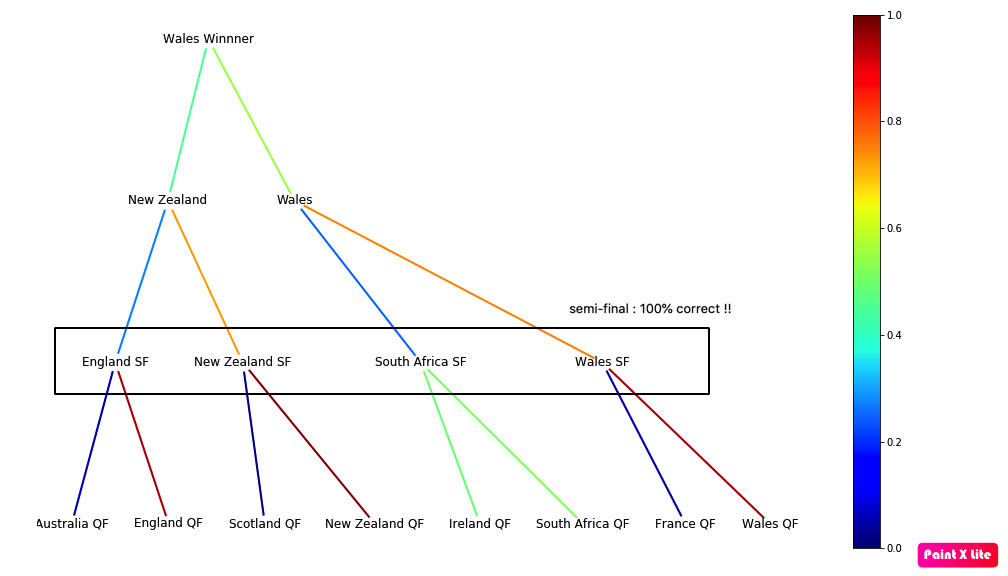
\includegraphics[trim={0 0 3.5cm 0}, clip, width=\textwidth]{fig/L3/predicting-rugby.png}
    \end{figure}
\end{frame}

\begin{frame}{But if we look at the easiest predictor....}
        \begin{figure}
        \centering
        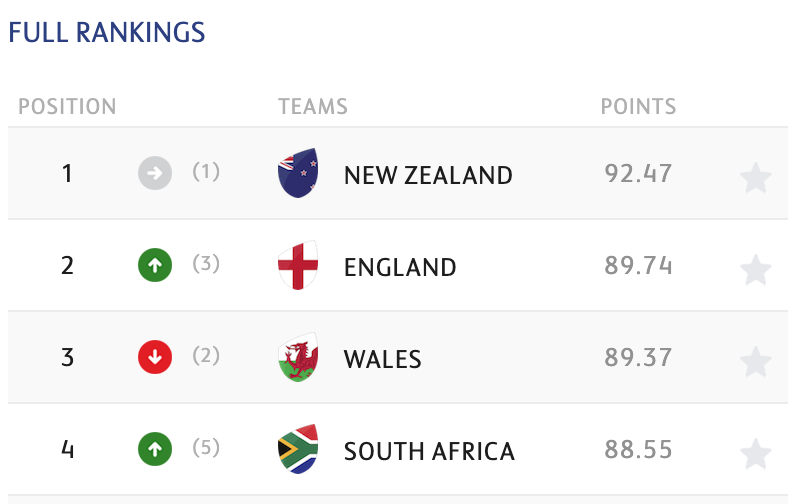
\includegraphics[width=\textwidth]{fig/L3/rugby-ranking.png}
    \end{figure}
\end{frame}

\begin{frame}{Table of contents}
  \setbeamertemplate{section in toc}[sections numbered]
  \tableofcontents[hideallsubsections]
\end{frame}

\section{Gradient backpropagation}
\begin{frame}{Training a neural-net: gradient backpropagation}

\begin{columns}

\column{.5\textwidth}
\begin{figure}
    \centering
 \begin{tikzpicture}[%
    node distance = 2.5em,
    basic/.style={draw,fill=blue!20,text width=1em,text badly centered},
    input/.style={basic,circle,fill=green!20},
    output/.style={basic,circle,fill=red!20},
    weights/.style={basic,rectangle},
functions/.style={basic,circle,fill=blue!10}
]
        \node[] (center) {};
        \node[right = of center, anchor = west,output] (right) {$\hat{y}$};
        \node[above of=center,functions] (h1) {$h_1$};
        \node[below of=center,functions] (h2) {$h_2$};
        \path[draw,->] (h1) -- node[above,midway]{$w^{1}_1$}(right);
        
        \path[draw,->] (h2) --  node[below,midway]{$w^{1}_2$}(right);
        
        \node[left = of h1, input] (x1) {$x_1$};
        \node[left = of h2, input] (x2) {$x_2$};
        
        \path [draw,->] (x1) -- node[above,midway]{$w^0_{11}$} (h1);
        \path [draw,->] (x1) -- node[pos=0.25,above]{$w^0_{12}$} (h2);
        \path [draw,->] (x2) -- node[pos=0.05,above]{$w^0_{21}$} (h1);
        \path [draw,->] (x2) -- node[below,midway]{$w^0_{22}$} (h2);
\end{tikzpicture}
\end{figure}
\begin{block}{Objective}
Determination of the best set of weights $\mathbf{w}$ to minimize the Loss function $L(\mathbf{w}) = ||\hat{y}(\mathbf{w})-y||^2$.\
\alert{Calculation of $\partial L/\partial w$}
\end{block}
\column{.6\textwidth}
\begin{enumerate}[<+->]
    \item Given a couple $(x,y)$
    \item \alert{Forward computation:}\\
    $h_j  =  f_0(\sum_{i=1}^2 w^0_{ij}.x_i)$\\
$\hat{y}  =  f_1(\sum_{j=1}^2 w^1_j. h_j)$
\item \alert{Compute the gradient of the loss:~}
$\boxed{\color{red}\partial L/\partial \hat{y}}$

    \item \alert{Gradient Backpropagation:}
    \begin{itemize}
   \item Layer 1\\
   $\alert{\partial L/\partial w_j^1} = 
   \boxed{\color{red}\partial L/\partial \hat{y}}.
   \partial f_1 / \partial w^1_j$\\
   
   $ \boxed{\color{blue}\partial L/\partial h_j} = 
    \boxed{\color{red}\partial L/\partial \hat{y}}. 
   \partial f_1 / \partial h_j$
   
   \item Layer 0\\
   $\alert{\partial L/\partial w^0_{ij}}=
  \boxed{\color{blue}\partial L/\partial h_j}
   .\partial f_1 / \partial w^0_{ij}  $
    
    \end{itemize}
\end{enumerate}

\end{columns}

\end{frame}

\section{Optimizing a machine learning (gradient method)}

\begin{frame}{Optimizing the loss}
    Several loss function (depending on the problem) can be defined.
    
    For example, Mean Square Error:
    
    \begin{alertblock}{Method}
    Find a minimum of L by adjustig the parameters (weights) $\mathbf{w}$ given the gradient of the loss with respect to the weights $\nabla_\mathbf{w}L$.
    \end{alertblock}
\end{frame}



\begin{frame}{Batch Vs Stochastic training}
Dataset: $(X,Y)$ with N samples denoted $(\mathbf{x_i},y_i)$

\begin{columns}[t]
\column{.56\textwidth}
\begin{footnotesize}
\begin{block}{Batch gradient:}\end{block}
    \begin{algorithmic}
    \Require{Learning rate(s): $\nu_k$}
    \Require{Initial weights: $\mathbf{w}$}
    \State $k \leftarrow 1$
    \While {stopping criterion not met}
   % \Require{NNNN}
    %\State Sample $m$ examples ($\mathbf{x}_i,y_i)$ from ($X,y$)
    \State Compute gradient: $\mathbf{g} \leftarrow \frac{1}{N}\sum_i^N\nabla_\mathbf{w}L(f(\mathbf{x}_i,y_i))$
    \State Update weights: $\mathbf{w} \leftarrow \mathbf{w} - \nu_k\mathbf{g}$
    \State $k \leftarrow k + 1$
    \EndWhile 
    \end{algorithmic}
    \end{footnotesize}
    \alert{1 Update / N forwards}
    \pause
    \column{.56\textwidth}
\begin{footnotesize}
\begin{block}{Stochastic gradient:}\end{block}
    \begin{algorithmic}
    \Require{Learning rate(s): $\nu_k$}
    \Require{Initial weights: $\mathbf{w}$}
    \State $k \leftarrow 1$
    \While {stopping criterion not met}
   % \Require{NNNN}
    %\State Sample $m$ examples ($\mathbf{x}_i,y_i)$ from ($X,y$)
    \State Sample an example ($\mathbf{x},y)$ from ($X,Y$)
    \State Compute gradient: $\mathbf{g} \leftarrow \nabla_\mathbf{w}L(f(\mathbf{x},y))$
    \State Update weights: $\mathbf{w} \leftarrow \mathbf{w} - \nu_k\mathbf{g}$
    \State $k \leftarrow k + 1$
    \EndWhile 
    \end{algorithmic}
    \end{footnotesize}
    \alert{1 Update / 1 forward}
    
    
    \end{columns}
\end{frame}

\begin{frame}{Mini-Batch training}
Dataset: $(X,y)$ with N samples
\begin{footnotesize}
\begin{block}{Mini-Batch gradient:}\end{block}

    \begin{algorithmic}
    \Require{Learning rate(s): $\nu_k$}
    \Require{Initial weights: $\mathbf{w}$}
    \State $k \leftarrow 1$
    \While {stopping criterion not met}
   % \Require{NNNN}
    \State Sample $m$ examples ($\mathbf{x}_i,y_i)$ from ($X,y$)
    \State Compute gradient: $\mathbf{g} \leftarrow \frac{1}{m}\sum_i^m\nabla_\mathbf{w}L(f(\mathbf{x}_i,y_i)$
    \State Update weights: $\mathbf{w} \leftarrow \mathbf{w} - \nu_k\mathbf{g}$
    \State $k \leftarrow k + 1$
    \EndWhile 
    
    \end{algorithmic}
    \end{footnotesize}
    \pause
        \alert{$m$ Update / 1 forward}\\
        $m=1$: Pure stochastic gradient.\\
        $m=N$: Batch gradient

\end{frame}


%%%%%%%%%%%%%%%%%%%%%%
\begin{frame}{Let's have a break}
\url{https://playground.tensorflow.org}
\end{frame}

\section{Other regularization techniques}
%%%%%%%%%%%%%%%%%%%%%
\begin{frame}{Regularization}
\begin{block}{Definition:}
\alert{Regularization} refers to the \alert{set of techniques} that \alert{constraints} the optimization. It is generally used to \alert{avoid overfitting}, but can also be used to inject prior knowledge during the training phase (e.g. set known limits to parameters)
\end{block}
\pause
\begin{itemize}
    \item Stochastic mini-batch gradient is a regularization technique
\end{itemize}

\end{frame}

%%%%%%%%%%%%%%%%%%%%%
\begin{frame}{Early Stopping}
    \begin{figure}
        \centering
        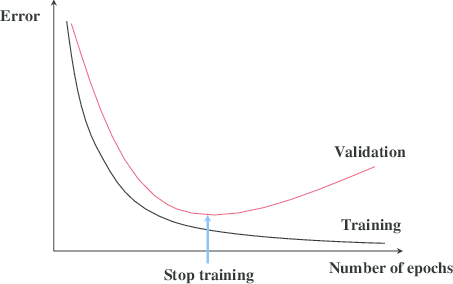
\includegraphics[width=\textwidth]{fig/L3/early_stopping.png}
    \end{figure}
\end{frame}
%%%%%%%%%%%%%%%%%%%%%
\begin{frame}{Dropout}
During training, randomly remove neurons on a layer with probability $p$.
 \begin{figure}
        \centering
\multiinclude[<+->][format=png,graphics={width=.6\textwidth}]{fig/L3/dropout}       
    \end{figure}
    \pause
    \begin{alertblock}{Practical remarks:}
    \begin{itemize}
        \item Avoid Dropout on convolutive layer
        \item Avoid Dropout on the last layer.
    \end{itemize}
    \end{alertblock}
    
    \end{frame}
    
    
\begin{frame}{Batch normalization}
From \textit{Ioffe et al. 2015, Batch normalizaion...}\\

Batch Normalization is a new type of layer.

If we use mini-batch training with a minibatch of size $m$:
\begin{columns}
\column{.8\textwidth}
\begin{footnotesize}
\begin{block}{Mini Batch Layer:}\end{block}
\renewcommand{\algorithmicrequire}{\textbf{Input:}}
\renewcommand{\algorithmicensure}{\textbf{Output:}}
    \begin{algorithmic}
    \Require{Values of $\mathbf{x_{1\dots m}}$}
    \Require{Initial parameters to be optimized: $\gamma, \beta$}
    \Ensure {$\mathbf{z_i} = {\rm BN}_{\gamma, \beta}(\mathbf{x}_i)$}
    \State $\mu \leftarrow \frac{1}{m}\sum_{i=1}^m \mathbf{x}_i$ \Comment{mini-batch mean}
    \State $\sigma^2 \leftarrow \frac{1}{m}\sum_{i=1}^m \left( \mathbf{x}_i - \mu \right)^2$ \Comment (mini-batch variance)
    \State $\hat{\mathbf{x}}_i \leftarrow (\mathbf{x}_i - \mu) / \sqrt{\sigma^2 + \epsilon}$ \Comment {normalize}
    \State $\mathbf{z_i} = \gamma \hat{\mathbf{x}}_i + \beta $ \Comment {Scale and shift}
    \State \Return $\mathbf{z_i}$
    \end{algorithmic}
    \end{footnotesize}

\end{columns}

$\mu$ and $\sigma^2$ are \alert{non-trainable parameters}. They are fixed for inferring new result (in test/validation).
\end{frame}

\section{Link with data assimilation}
\begin{frame}{Data Assimilation}
   Example of \textcolor{blue}{BLUE}{: Best Linear Unbiased Estimator}
    
    Given a state vector $\mathbf{x}\in \mathbb{R}^n$ and a data vector  $\mathbf{d}\in \mathbb{R}^m$:
\begin{tabular}{p{.3\textwidth}p{.2\textwidth}p{.2\textwidth}}
    $\mathbf{x}^{\rm f} = \mathbf{x}^{\rm t} + \mathbf{p},$ & $\overline{\mathbf{p}}=0,$ &$ \overline{\mathbf{p}\mathbf{p}^T} = \mathbf{C}_{xx}.$\\
    $\mathbf{d} = \mathbf{H}\mathbf{x}^{\rm t} + \boldsymbol{\epsilon},$ & $\overline{\boldsymbol{\epsilon}}=0,$ & $ \overline{\boldsymbol{\epsilon}\boldsymbol{\epsilon}^T} = \mathbf{C}_{\epsilon \epsilon}.$
    
    \end{tabular}
    \pause
    Estimating $\mathbf{x}^{\rm t}$ by minimizing the estimation error leads to minizing the following function:
    \begin{equation*}
        \mathcal{J}(\mathbf{x}) = 
          (\mathbf{d} - \mathbf{H}\mathbf{x})^T  \mathbf{C}_{\epsilon \epsilon}^{-1}  (\mathbf{d} - \mathbf{H}\mathbf{x}) + (\mathbf{x} - \mathbf{x}^{\rm f})^T \mathbf{C}^{-1}_{xx}(\mathbf{x} - \mathbf{x}^{\rm f})
    \end{equation*}
    \pause
    \begin{alertblock}{This is data assimilation!}
    We correct a forecast $\mathbf{x}^{\rm f}$ given some observational data $\mathbf{d}$
    \end{alertblock}
\end{frame}

\begin{frame}{Is it machine learning?}
\begin{footnotesize}

    \begin{itemize}
        \item Ridge regression: $
J(\bm{\theta}) =(\mathbf{y} - h_{\bm{\theta}}(\mathbf{x}))^T (\mathbf{y} - h_{\bm{\theta}}(\mathbf{x})) + \alpha  \theta^T \theta
$
\item BLUE:  $\mathcal{J}(\mathbf{x}) = 
          (\mathbf{d} - \mathbf{H}\mathbf{x})^T  \mathbf{C}_{\epsilon \epsilon}^{-1}  (\mathbf{d} - \mathbf{H}\mathbf{x}) + (\mathbf{x} - \mathbf{x}^{\rm f})^T \mathbf{C}^{-1}_{xx}(\mathbf{x} - \mathbf{x}^{\rm f})$
    \end{itemize}
    \end{footnotesize}
    \pause
    \begin{table}[]
        \centering
        \begin{tabular}{c|c}
            BLUE & Ridge \\
            \hline
            data $\mathbf{d}$ & target $\mathbf{y}$  \\
            Observation operator $\mathbf{H}$ & feature $\mathbf{x}$ \\
            State $\mathbf{x}$ & parameters $\bm{\theta}$\\
            $\mathbf{C}_{\epsilon \epsilon} \mathbf{C}^{-1}_{xx}$ & $\alpha$
        \end{tabular}
    \end{table}
    \pause
    \begin{block}{Further links...}
    If a numerical model is integrated over several time steps, it can be related to successive layers of a Neural Network.
    \end{block}
\end{frame}

%%%%%%%%%%%%%%%%%%
\begin{frame}[fragile]{Questions addressed in this lecture}
    \begin{itemize}
        \item What is gradient backpropagation? [GBC16,6]
        \item What are the different types of gradient descent techniques? [GBC16,8]
        \item What are some other types of regularizations? [GBC16,7]
        \item How machine learning can be related to data assimilation?
        \item Who is going to win the next Rugby world cup? 
    \end{itemize}

\begin{footnotesize}
\begin{block}{Refs}
~[Van16,$n$]: Jake VanderPlas, \textit{Python Data Science Handbook}, section $n$\\
~[GBC16,$n$]: Goodfellow etal., Deep Learning, chapter $n$
\end{block}
\end{footnotesize}
\end{frame}
%%%%%%%%%%%%%%%%%%%%%
%%%%%%%%%%%%%%%%%%%%%
%%%%%%%%%%%%%%%%%%%%%
%%%%%%%%%%%%%%%%%%%%%
%%%%%%%%%%%%%%%%%%%%%%%%%%%%%%%%%%%%%%%%%%
%%%%%%%%%%%%%%%%%%%%%
%%%%%%%%%%%%%%%%%%%%%%%%%%%%%%%%%%%%%%%%%%
\end{document}
%%%%%%%%%%%%%%%%%%%%%%%%%%%%%%%%%%%%%%%%%%



%%%%%%%%%%%%%%%%%%%%%
\begin{frame}
\frametitle{Model Selection}
\begin{alertblock}{The "big" question}
How to determine some "hyper-parameter" of our model ?

examples: $\alpha$ for regularization, degree of polynomials
\end{alertblock}
\pause
The common approach:
\begin{enumerate}[<+->]
\item Split the dataset in two dataset : training and test
\item Optimize the parameters on the training dataset for a range of models (e.g. several values of $\alpha$)
\item Select the model with a lowest error on the test dataset
\end{enumerate}
\end{frame}
 
%%%%%%%%%%%%%%%%%%%%%
\begin{frame}
\frametitle{Test dataset}
\begin{columns}
\column{.5\textwidth}
\begin{figure}
The dataset:\\
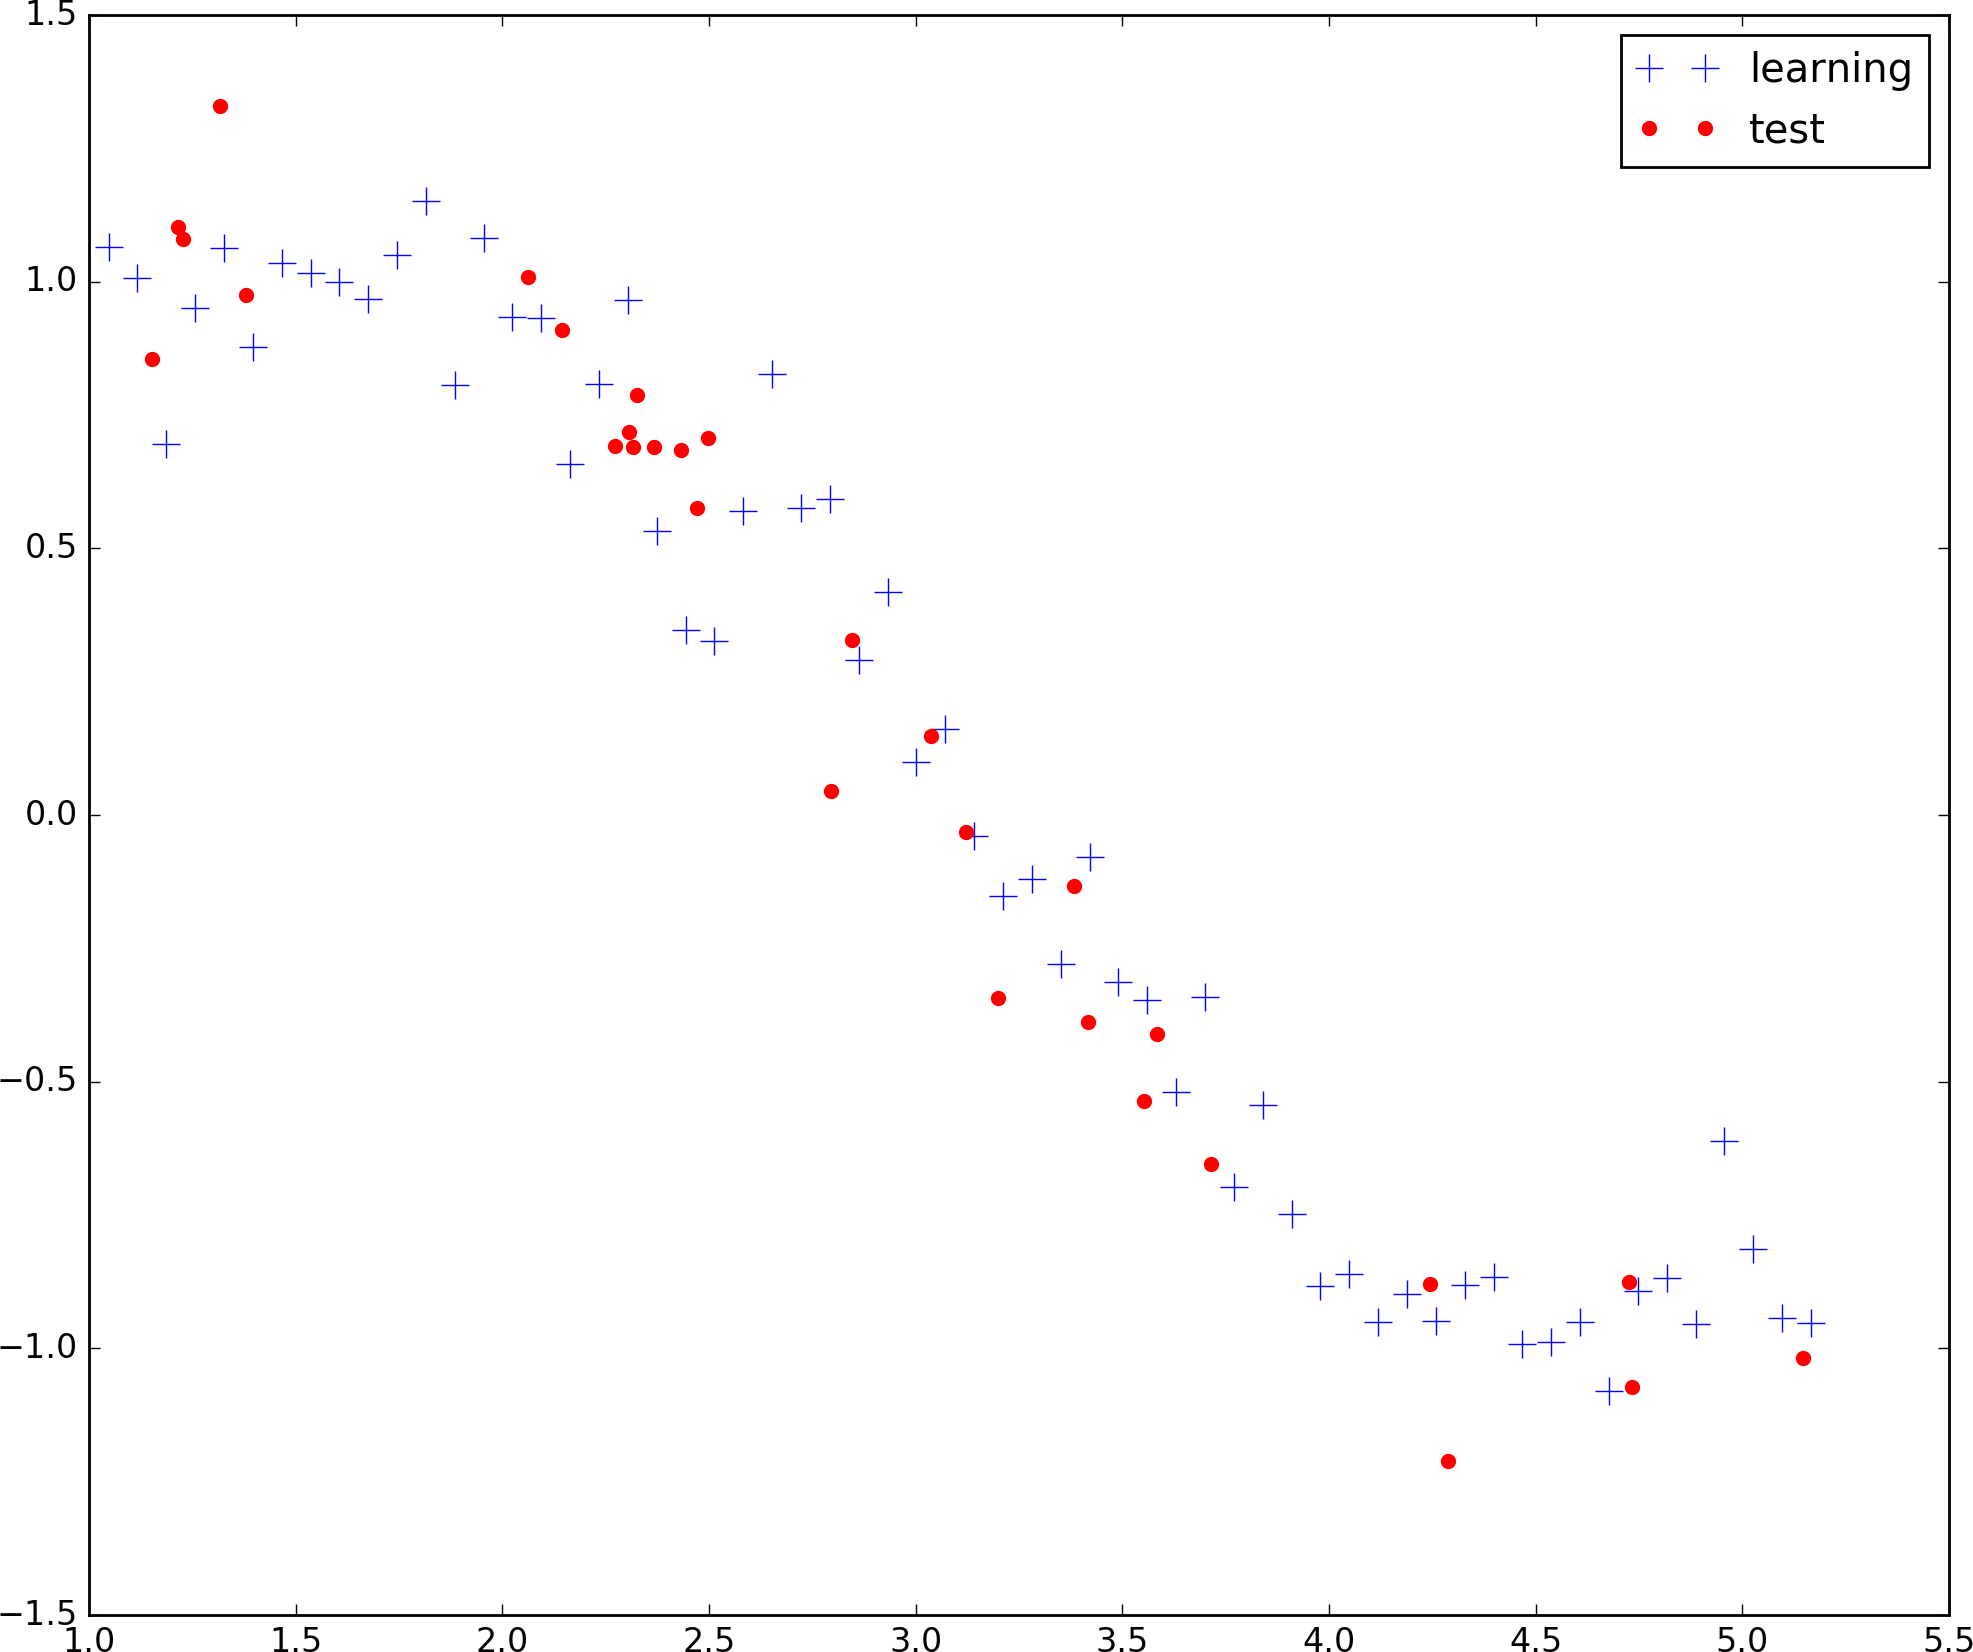
\includegraphics[width=\textwidth]{./fig/L1/scatter_test.png}
\end{figure}
\pause
\column{.5\textwidth}
\begin{figure}
Error on the training and the test
with respect with $\alpha$
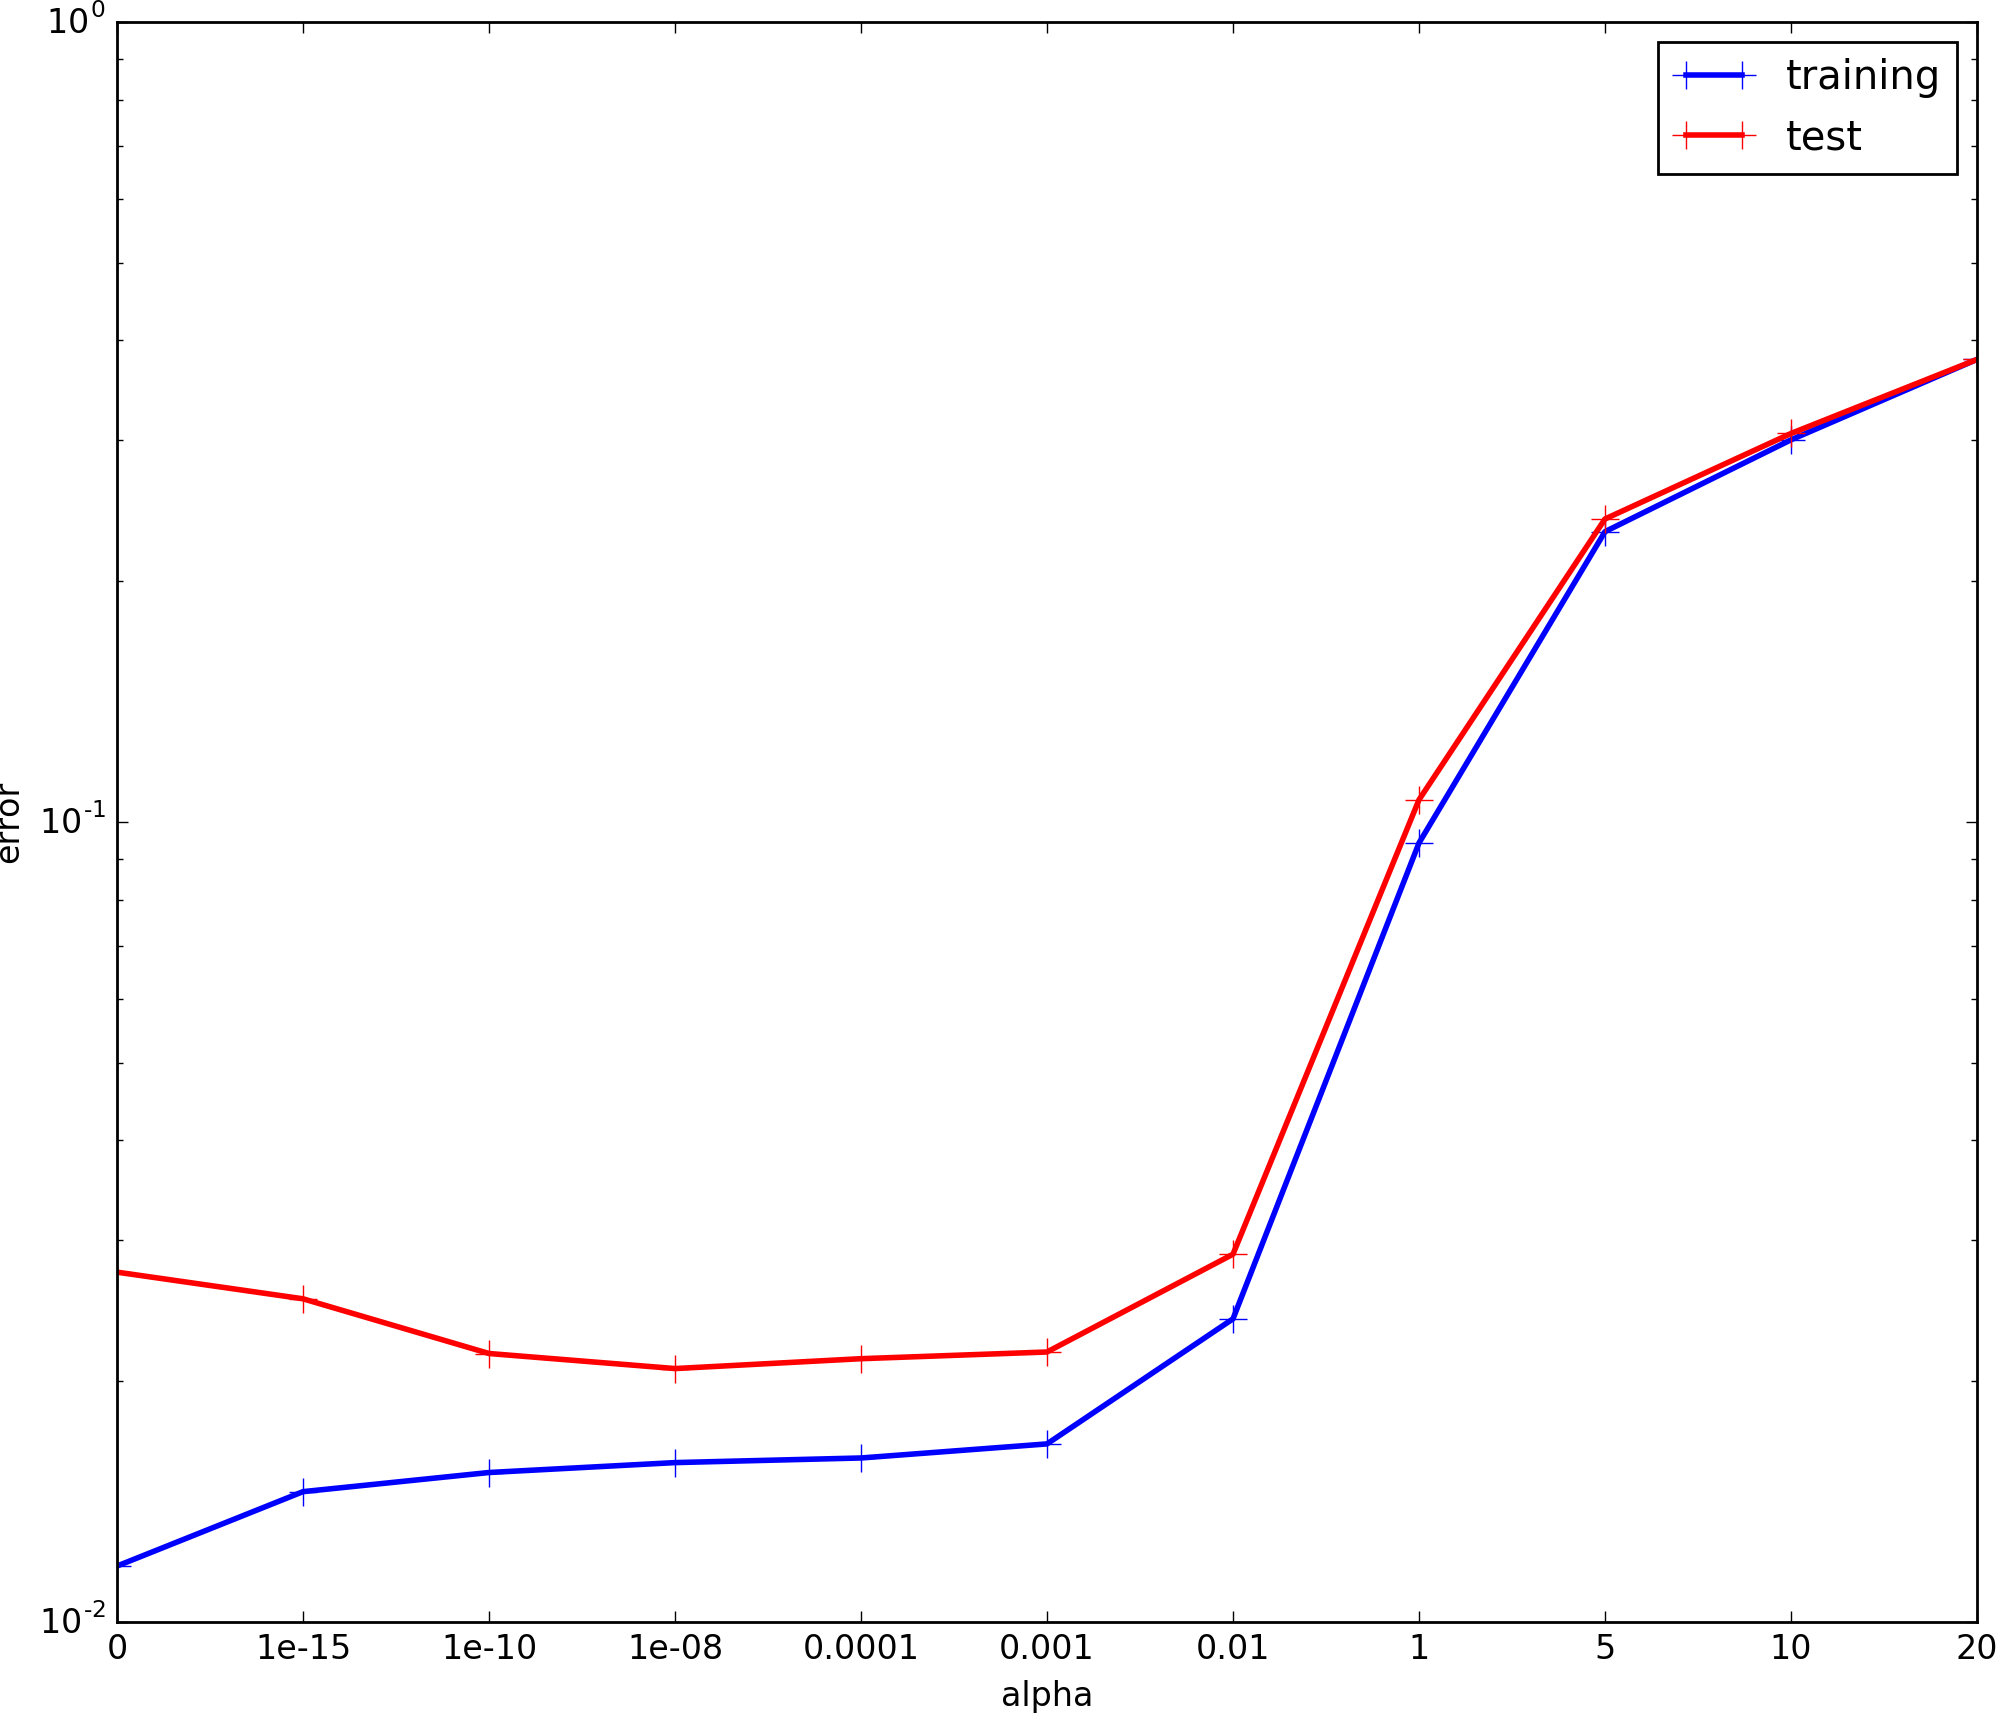
\includegraphics[width=\textwidth]{./fig/L1/validation.png}
\end{figure}

\end{columns}
\end{frame}



\begin{frame}
  \frametitle{Introduction to the percpetron}
  \begin{block}{}
  Introduced by Frank Rosenblatt ( July 11, 1928 - July 11, 1971) in 1957
  \end{block}
  \pause
  \begin{figure}
  \begin{tikzpicture}[
    basic/.style={draw,fill=blue!20,text width=1em,text badly centered},
    input/.style={basic,circle},
    weights/.style={basic,rectangle},
functions/.style={basic,circle,fill=blue!10},
]
        \node[functions] (center) {};
        \node[below of=center,font=\scriptsize,text width=4em] {Activation function};
        \draw[thick] (0.5em,0.5em) -- (0,0.5em) -- (0,-0.5em) -- (-0.5em,-0.5em);
      %  \draw (0em,0.75em) -- (0em,-0.75em);
      %  \draw (0.75em,0em) -- (-0.75em,0em);
        \node[right of=center, anchor = west] (right) {$y=$ 0 ou 1};
            \path[draw,->] (center) -- (right);
        \node[functions,left=3em of center] (left) {$\sum$};
            \path[draw,->] (left) -- (center);
%        \node[weights,left=3em of left] (2) {$w_2$} -- (2) 
            \node[input,left= 4em of left] (l2) {$x_2$};
%            \path[draw,->] (l2) -- (2);
            \path[draw,->] (l2) -- node[above,midway]{$w_2$}(left);
        \node[below of=l2] (dots) {$\vdots$} ;
%(dots) node[left of=dots] (ldots) {$\vdots$};
%        \node[weights,below of=dots] (n) {$w_n$} -- (n) 
\node[input,below of=dots] (ln) {$x_n$};
%            \path[draw,->] (ln) -- (n);
            \path[draw,->] (ln) -- node[above,midway]{$w_n$}(left);
%        \node[weights,above of=2] (1) {$w_1$} -- (1) 
            \node[input,above of=l2] (l1) {$x_1$};
%            \path[draw,->] (l1) -- (1);
            \path[draw,->] (l1) -- node[above,midway]{$w_1$}(left);
%        \node[weights,above of=1] (0) {$w_0$} -- (0) 
\node[input,above of=l1] (l0) {$1$};
%            \path[draw,->] (l0) -- (0);
            \path[draw,->] (l0) -- node[above,midway]{$w_0$}(left);
        \node[below of=ln,font=\scriptsize](lin) {inputs};
        \node[right of=lin,font=\scriptsize] {weights};
    \end{tikzpicture}
    \end{figure}
\begin{block}{}
If $w_0 + w_1 x_1 + w_2 x_2 +  \dots + w_n\ x_n < 0$, then $y=0$\\
else $y=1$
\end{block}
\end{frame}
\begin{frame}
\frametitle{Two different predictions}

\begin{columns}
\column{0.45\textwidth}
$w_0=$ \red{1}, $w_1=$ \red{-2},$w_2=$ \red{2}\\
\vspace{1em}

 \begin{tikzpicture}[
    basic/.style={draw,fill=blue!20,text width=1em,text badly centered},
    input/.style={basic,circle, text width=1em, inner sep=0},
    weights/.style={basic,rectangle},
functions/.style={basic,circle,fill=blue!10},
]
        \node[functions] (center) {};
        \draw[thick] (0.5em,0.5em) -- (0,0.5em) -- (0,-0.5em) -- (-0.5em,-0.5em);
        \node[right = 1em of center, anchor = west] (right) {$y=$ \red{1}};
            \path[draw,->] (center) -- (right);
        \node[functions,left=1em of center] (left) {$\sum$};
            \path[draw,->] (left) -- (center);
            \node[left= 2em of left] (l2) {$x_1=0$};
            \path[draw,->] (l2) -- node[above,midway]{$w_1$}(left);
            \node[below of=l2] (ln) {$x_2=1$};
            \path[draw,->] (ln) -- node[above,midway]{$w_2$}(left);
            \node[above of=l2] (l1) {$1$};
            \path[draw,->] (l1) -- node[above,midway]{$w_0$}(left);
           % \node[input,above of=l1] (l0) {$1$};
           % \path[draw,->] (l0) -- node[above,midway]{$w_0$}(left);
%        \node[below of=ln,font=\scriptsize](lin) {inputs};
%        \node[right of=lin,font=\scriptsize] {weights};
    \end{tikzpicture}

$$
w_0 + w_1 x_1 + w_2 x_2 = 3 > 0
$$

\column{0.45\textwidth}
$w_0=$ \red{1}, $w_1=$ \red{2},$w_2=$ \red{-2}\\
\vspace{1em}

 \begin{tikzpicture}[
    basic/.style={draw,fill=blue!20,text width=1em,text badly centered},
    input/.style={basic,circle, text width=1em, inner sep=0},
    weights/.style={basic,rectangle},
functions/.style={basic,circle,fill=blue!10},
]
        \node[functions] (center) {};
        \draw[thick] (0.5em,0.5em) -- (0,0.5em) -- (0,-0.5em) -- (-0.5em,-0.5em);
        \node[right = 1em of center, anchor = west] (right) {$y=$ \red{0}};
            \path[draw,->] (center) -- (right);
        \node[functions,left=1em of center] (left) {$\sum$};
            \path[draw,->] (left) -- (center);
            \node[left= 2em of left] (l2) {$x_1=0$};
            \path[draw,->] (l2) -- node[above,midway]{$w_1$}(left);
            \node[below of=l2] (ln) {$x_2=1$};
            \path[draw,->] (ln) -- node[above,midway]{$w_2$}(left);
            \node[above of=l2] (l1) {$1$};
            \path[draw,->] (l1) -- node[above,midway]{$w_0$}(left);
           % \node[input,above of=l1] (l0) {$1$};
           % \path[draw,->] (l0) -- node[above,midway]{$w_0$}(left);
%        \node[below of=ln,font=\scriptsize](lin) {inputs};
%        \node[right of=lin,font=\scriptsize] {weights};
    \end{tikzpicture}

$$
w_0 + w_1 x_1 + w_2 x_2 = -1 < 0
$$

\end{columns}


\end{frame}

\begin{frame}
\frametitle{Learning of the weights}
\framesubtitle{Supervised learning}
Training set: $\{(x_1,y_1),\ldots,(x_n,y_n)\}$

\begin{block}{Learning algorithm}
\begin{enumerate}[<+->]
\item Initialization of the weights $w_i$
\item We consider the data $(x_j,y_j)$
\item The perceptron predicts $\hat{y}_j$
\item Update of the weights:\\
$w_i=w_i- (\hat{y}_j - y_j)\times x_{ij}$
\item Back to step 2
\end{enumerate}
\end{block}

\end{frame}

\begin{frame}
\frametitle{Link between perceptron and Linear/logistic regression}

\begin{itemize}
\item weight in a perceptron $\Leftrightarrow$ parameters of a model
\item Activation function  $\Leftrightarrow$ hypothesis model
\item If the activation function is linear, perceptron performs a linear regression
\item If the activation function is a sigmoid, perceptron performs a logistic regression
\end{itemize}

\end{frame}
